Software engineering requires rigorous testing of rapidly evolving programs,
which costs manpower comparable to developing the product itself~\cite{vailshery}.  To guarantee
programs' compliance with their specifications, we need testers that can tell
compliant implementations from violating ones.

This thesis studies the testing of interactive systems' semantics: The system
under test (SUT) interacts with the tester by sending and receiving messages,
and the tester determines whether the messages sent by the SUT are valid
with respect to the protocol specification.

This chapter provides a brief view of interactive testing
(\autoref{sec:interactive-testing}), explains why nondeterminism makes this
problem difficult
(Sections~\ref{sec:internal-external-nondeterminism}--\ref{sec:inter-execution-nondeterminism}),
discusses the field of existing works (\autoref{sec:existing-work}), and
summarizes the contributions of this thesis in addressing the challenges caused
by nondeterminism (\autoref{sec:contribution}).

\section{Interactive Testing}
\label{sec:interactive-testing}
Suppose we want to test a web server that supports GET and PUT methods.  The
server is a stateful program written as a recursive function:\footnote{Syntax
``\ilc{x <- f;; y}'' encodes a monadic program that binds the result of
computation \ilc f as variable \ilc x in continuation \ilc y.  For example, to
receive a request is to bind the result of \ilc{recv} as variable \ilc{request}
in the remaining program that performs pattern matching on it.}\footnote{Syntax
``\ilc{data [k|->v]}'' represents a key-value store where \ilc k is mapped
to \ilc v, and all other keys are mapped by \ilc{data}.  That is, for
all \ilc{k'} that are not equal to \ilc k, \ilc{(data [k|->v]) k'} is equal
to \ilc{(data k')}.}
\begin{coq}
  CoFixpoint server (data: key -> value) :=
    request <- recv;;
    match request with
    | GET k   => send (data k);; server  data
    | PUT k v => send  Done   ;; server (data [k |-> v])
    end.
\end{coq}
Here the \ilc{server} function iterates over a parameter called \ilc{data},
which is a key-value store.  In each iteration, the server receives a request
and computes its response.  It then sends back the response and recurses with
the updated data.

We can write a tester client that interacts with the server and determines
whether it behaves correctly:
\begin{coq}
  CoFixpoint tester (data: key -> value) :=
    request <- random;;
    send request;;
    response <- recv;;
    match request with
    | GET k   => if response =? data k
                 then tester data
                 else reject
    | PUT k v => if response =? Done
                 then tester (data [k |-> v])
                 else reject
    end.
\end{coq}
This tester implements a reference server internally that computes the expected
behavior.  The behavior is then compared against that produced by the SUT.  The
tester rejects the SUT upon any difference from the computed expectation.

The above tester can be viewed as two modules: (i) a {\em test harness} that
interacts with the server and produces transactions of sends and receives, and
(ii) a {\em validator} that determines whether the transactions are valid or
not:
\begin{coq}
  (* Compute the expected response and next state of the server. *)
  Definition serverSpec request data :=
    match request with
    | GET k   => (data k, data)
    | PUT k v => (Done  , data [k |-> v])
    end.

  (* Validate the transaction against the stateful specification. *)
  Definition validate spec request response data :=
    let (expect, next) := spec request data in
    if response =? expect then Success next else Failure.

  (* Produce transactions for the validator. *)
  CoFixpoint harness validator state :=
    request <- random;;
    send request;;
    response <- recv;;
    if validator request response state is Success next
    then harness validator next
    else reject.

  Definition tester := harness (validate serverSpec).
\end{coq}
This testing method works for deterministic systems, whose behavior can be
precisely computed from their inputs.  But, many systems are allowed to behave
nondeterministically.  For example, systems may implement various hash
algorithms, or buffer network packets in different ways.  The following sections
discuss nondeterminism by partitioning it in two ways, and explains how they
pose challenges to the validator and the test harness.

\section{Internal and external nondeterminism}
\label{sec:internal-external-nondeterminism}
When people talk to each other, voice is transmitted over substances like air or
metal.  When testers interact with the SUT, messages are transmitted via the
runtime environment.  The specification might allow SUTs to behave differently
from each other, just like people speaking in different accents; we call it {\em
internal nondeterminism}.  The runtime environment might affect the transmission
of messages, just like solids transmit voice faster than liquids and gases; we
call it {\em external nondeterminism}.

\subsection{Internal nondeterminism}
\label{sec:internal-nondeterminism}
Within the SUT, correct behavior may be \mbox{underspecified}.  Consider web
browsing as an example: If a client has cached a local copy of some resource,
then when fetching updates for the resource, the client can ask the server not
to send the resource's contents if it is the same as the cached copy.  To
achieve this, an HTTP server may generate a short string, called an ``entity
tag'' (ETag)~\cite{rfc7232}, identifying the content of some resource, and send
it to the client:
\begin{center}
  \begin{minipage}[t]{.4\textwidth}
    \begin{cpp}
/* Client: */
GET /target HTTP/1.1
    \end{cpp}
  \end{minipage}\begin{minipage}[t]{.4\textwidth}
    \begin{cpp}
/* Server: */
HTTP/1.1 200 OK
ETag: "tag-foo"
... content of /target ...
    \end{cpp}
  \end{minipage}
\end{center}
The next time the client requests the same resource, it can include the ETag in
the GET request, informing the server not to send the content if its ETag still
matches:
\begin{center}
\begin{minipage}[t]{.4\textwidth}
\begin{cpp}
/* Client: */
GET /target HTTP/1.1
If-None-Match: "tag-foo"
\end{cpp}
\end{minipage}\begin{minipage}[t]{.4\textwidth}
\begin{cpp}
/* Server: */
HTTP/1.1 304 Not Modified
\end{cpp}
\end{minipage}
\end{center}
If the ETag does not match, the server responds with code 200 and the updated
content as usual.

Similarly, if a client wants to modify the server's resource atomically by
compare-and-swap, it can include the ETag in the PUT request as an
\inlinec{If-Match} precondition, which instructs the server to only update the
content if its current ETag matches:
\begin{center}
  \begin{minipage}[t]{.4\textwidth}
    \begin{cpp}
/* Client: */
PUT /target HTTP/1.1
If-Match: "tag-foo"
... content (A) ...
    \end{cpp}
  \end{minipage}
  \begin{minipage}[t]{.4\textwidth}
    \begin{cpp}
/* Server: */
HTTP/1.1 204 No Content
    \end{cpp}
  \end{minipage}

  \begin{minipage}[t]{.4\textwidth}
    \begin{cpp}
/* Client: */
GET /target HTTP/1.1
    \end{cpp}
  \end{minipage}
  \begin{minipage}[t]{.4\textwidth}
    \begin{cpp}
/* Server: */
HTTP/1.1 200 OK
ETag: "tag-bar"
... content (A) ...
    \end{cpp}
  \end{minipage}
\end{center}
If the ETag does not match, then the server should not perform the requested
operation, and should reject with code 412:
\begin{center}
  \begin{minipage}[t]{.4\textwidth}
    \begin{cpp}
/* Client: */
PUT /target HTTP/1.1
If-Match: "tag-baz"
... content (B) ...
    \end{cpp}
  \end{minipage}
  \begin{minipage}[t]{.4\textwidth}
    \begin{cpp}
/* Server: */
HTTP/1.1 412 Precondition Failed
    \end{cpp}
  \end{minipage}

  \begin{minipage}[t]{.4\textwidth}
    \begin{cpp}
/* Client: */
GET /target HTTP/1.1
    \end{cpp}
  \end{minipage}
  \begin{minipage}[t]{.4\textwidth}
    \begin{cpp}
/* Server: */
HTTP/1.1 200 ok
ETag: "tag-bar"
... content (A) ...
    \end{cpp}
  \end{minipage}
\end{center}
Whether a server's response should be judged {\em valid} or not depends on the
ETag it generated when creating the resource.  If the tester doesn't know the
server's internal state ({\it e.g.}, before receiving any 200 response that
includes an ETag), and cannot enumerate all of them (as ETags can be arbitrary
strings), then it needs to maintain a space of all possible values, and narrow
the space upon further interactions with the server.  For example, ``If the
server has revealed some resource's ETag as \inlinec{"tag-foo"}, then it must
not reject requests targeting this resource conditioned over \inlinec{If-Match:
  "tag-foo"}, until the resource has been modified''; and ``Had the server
previously rejected an \inlinec{If-Match} request, it must reject the same
request until its target has been modified.''

\begin{figure}
\begin{coq}
  Definition validate request response
             (data      : key -> value)
             (tag_is    : key -> Maybe etag)
             (tag_is_not: key -> list etag) :=
    match request, response with
    | PUT k t v, NoContent => 
      if t \in tag_is_not k then Failure
      else if (tag_is k =? Unknown) || strong_match (tag_is k) t
      then (* Now the tester knows that the data in [k]
            * is updated to [v], but its new ETag is unknown. *)
        Success (data       [k |-> v],
                 tag_is     [k |-> Unknown],
                 tag_is_not [k |-> [] ])
      else Failure
    | PUT k t v, PreconditionFailed =>
      if strong_match (tag_is k) t then Failure
      else (* Now the tester knows that the ETag of [k]
            * is other than [t]. *)
        Success (data, tag_is, tag_is_not [k |-> t::(tag_is_not k)])
    | GET k t, NotModified =>
      if t \in tag_is_not then Failure
      else if (tag_is k =? Unknown) || weak_match (tag_is k) t
      then (* Now the tester knows that the ETag of [k]
            * is equal to [t]. *)
        Success (data, tag_is [k |-> Known t], tag_is_not)
      else Failure
    | GET k t0, OK t v =>
      if weak_match (tag_is k) t0 then Failure
      else if data k =? v
      then (* Now the tester knows the ETag of [k]. *)
        Success (data, tag_is [k |-> Known t], tag_is_not)
      else Failure
    | _, _ => Failure
    end.
\end{coq}
  \caption[Ad hoc tester for \http conditional requests.]{Ad hoc tester for
    \http conditional requests.  \ilc{PUT k t v} represents a PUT request that
    changes \ilc k's value into \ilc v only if its ETag matches \ilc t; \ilc{GET
      k t} is a GET request for \ilc k's value only if its ETag does not match
    \ilc t; \ilc{OK t v} indicates that the request target's value is \ilc v and
    its ETag is \ilc t.}
  \label{fig:etag-tester}
\end{figure}

This idea of remembering matched and mismatched ETags is implemented in
\autoref{fig:etag-tester}.  For each key, the validator maintains three internal
states: (i) The value stored in \ilc{data}, (ii) the corresponding resource's
ETag, if known by the tester, stored in \ilc{tag_is}, and (iii) ETags that are
known to not match the resource's, stored in \ilc{tag_is_not}.  Each pair of
request and response contributes to the validator's knowledge of the target
resource.  The tester rejects the SUT if the observed behavior does not match
the knowledge gained in previous interactions.

Even simple nondeterminism like ETags requires such careful design of the
validator, based on thorough comprehension of the specification.  We need to
construct the validator in a scalable way for more complex protocols.

\subsection{External nondeterminism}
\label{sec:intro-external-nondet}
To discuss the nondeterminism caused by the environment, we need to define the
environment concept in testing scenario.
\begin{definition}[Environment, input, output, and observations]
  {\em Environment} is the substance that the tester and the SUT interact with.
  {\em Input} is the subset of the environment that the tester can manipulate.
  {\em Output} is the subset of the environment that the SUT can alter.  {\em
    Observation} is the tester's view of the environment.
\end{definition}
When testing servers, the environment is the network stack between the client
and the server.  The input is the sequence of requests sent by the client, and
the output is the sequence of responses sent by the server.  The responses are
transmitted via the network, until reaching the client side as observations.

\begin{figure}
  \centering
  \begin{minipage}[c]{.3\textwidth}
\begin{coq}
  (* Observation: *)
  1> PUT k "new"
  1< Done
  2> GET k
  2< "new"
\end{coq}
  \end{minipage}\begin{minipage}[c]{.4\textwidth}
  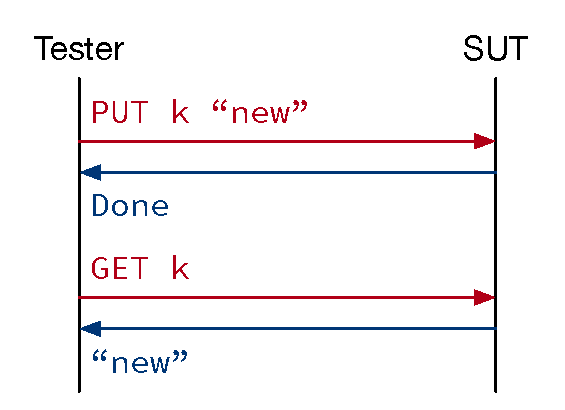
\includegraphics[width=\linewidth]{figures/linear-trace}
  \end{minipage}\begin{minipage}[c]{.3\textwidth}
\begin{coq}
  (* Output: *)
  1> PUT k "new"
  1< Done
  2> GET k
  2< "new"
\end{coq}
  \end{minipage}
  \caption[Linear trace with no concurrency.]{With no concurrency, the
    observation is identical to the output.}
  \label{fig:linear-trace}
\end{figure}
\begin{figure}
  \centering
  \begin{minipage}[c]{.3\textwidth}
\begin{coq}
  (* Observation: *)
  1> PUT k "new"
  2> GET k
  1< Done
  2< "old"
\end{coq}
  \end{minipage}\begin{minipage}[c]{.4\textwidth}
    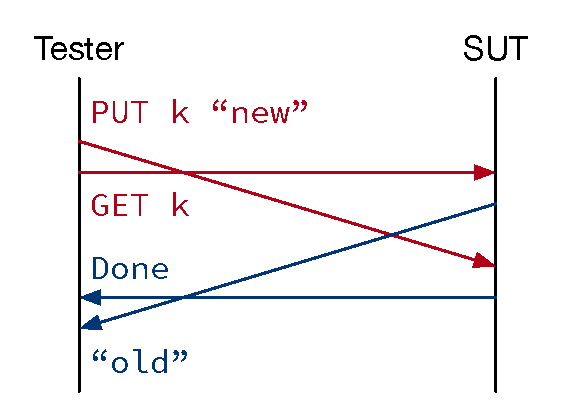
\includegraphics[width=\linewidth]{figures/network-trace}
  \end{minipage}\begin{minipage}[c]{.3\textwidth}
\begin{coq}
  (* Output: *)
  2> GET k
  2< "old"
  1> PUT k "new"
  1< Done
\end{coq}
  \end{minipage}
  \caption[Reordered trace upon network delays.]{Acceptable: The observation can
    be explained by a valid output reordered by the network environment.}
  \label{fig:reordered-trace}
\end{figure}
\begin{figure}
  \centering
  \begin{minipage}[c]{.3\textwidth}
\begin{coq}
  (* Observation: *)
  1> PUT k "new"
  1< Done
  2> GET k
  2< "old"
\end{coq}
  \end{minipage}\begin{minipage}[c]{.4\textwidth}
  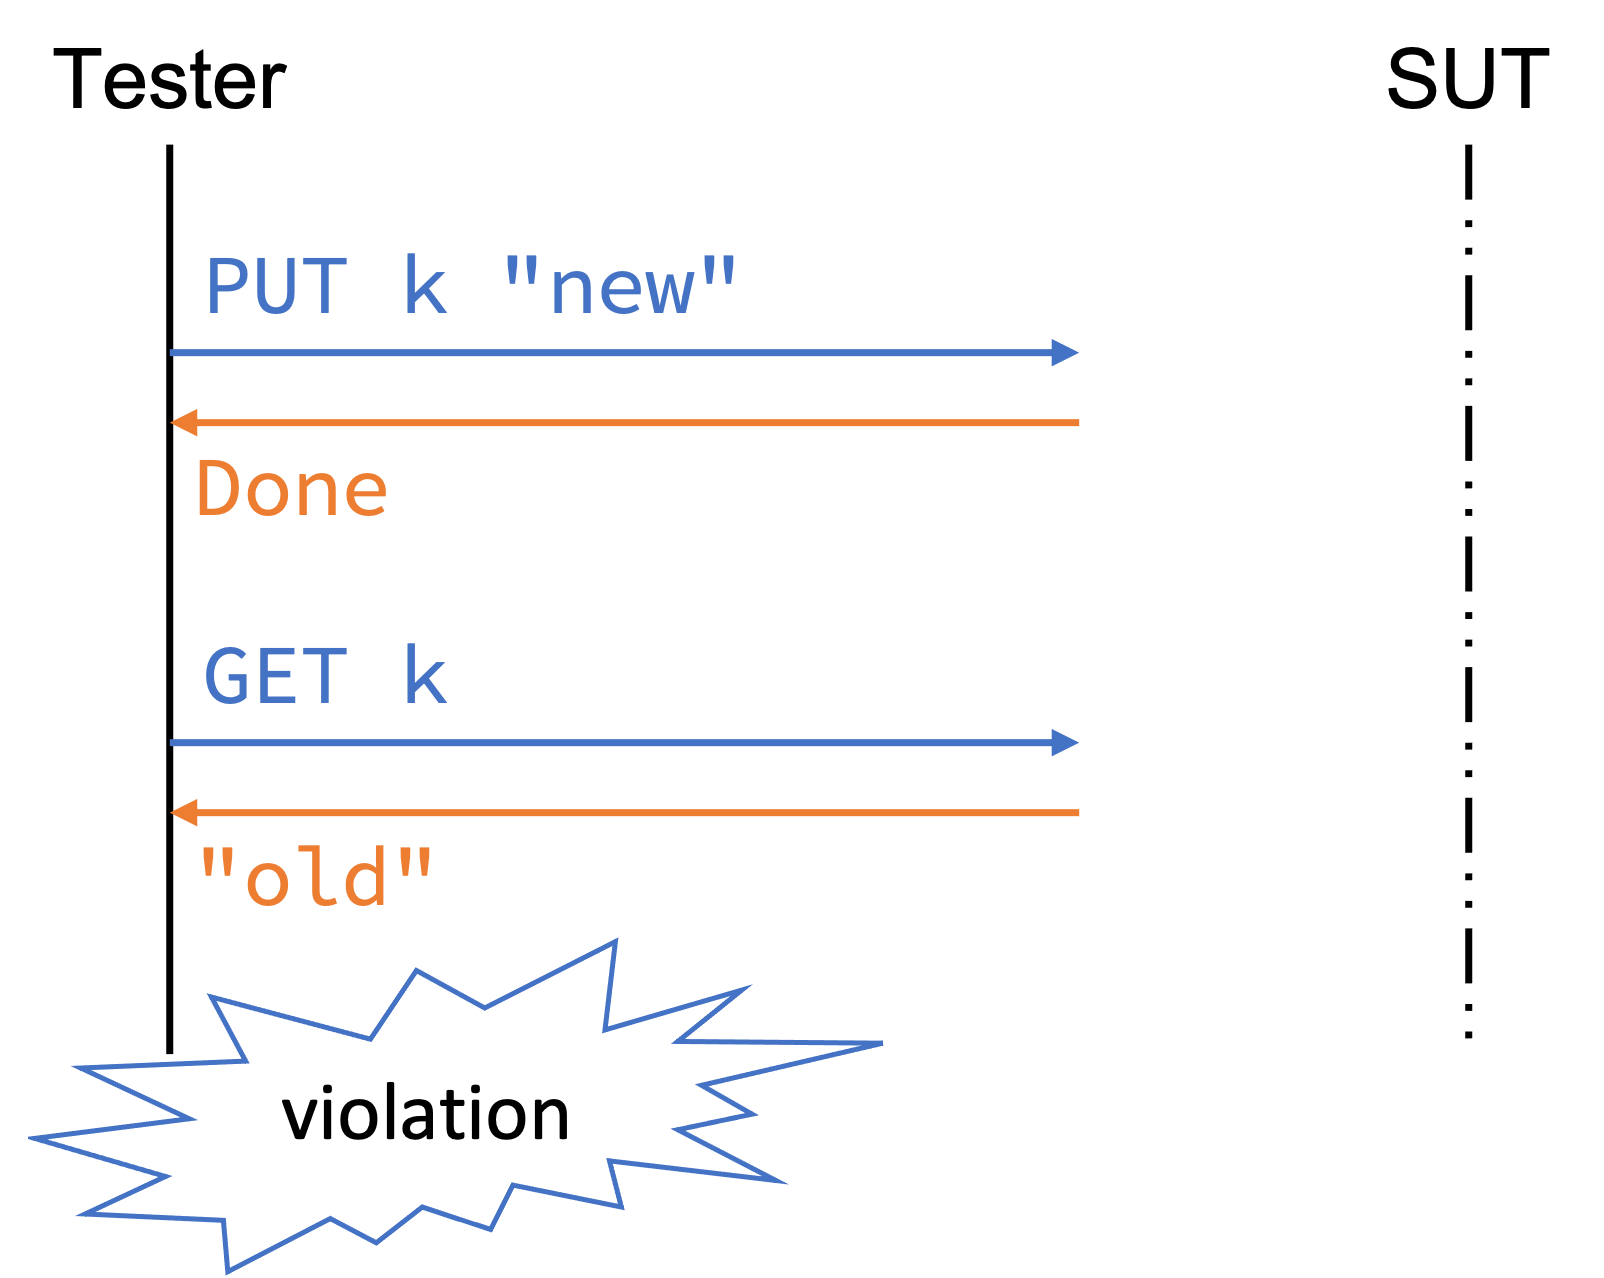
\includegraphics[width=\linewidth]{figures/invalid-trace}
  \end{minipage}\begin{minipage}[c]{.3\textwidth}\
  \end{minipage}
  \caption[Invalid trace that violates the specification.]{Unacceptable: The
    tester received the \ilc{Done} response before sending the \ilc{GET}
    request, thus the SUT must have processed the \ilc{PUT} request before the
    \ilc{GET} request.  Therefore, the \ilc{"old"} response is invalid.}
  \label{fig:invalid-trace}
\end{figure}
The tester shown in \autoref{sec:interactive-testing} runs one client at a time.
It waits for the response before sending the next request, as shown in
\autoref{fig:linear-trace}.  Such tester's observation is guaranteed identical
to the SUT's output, so it only needs to scan the requests and responses with
one stateful validator.

To reveal the server's behavior upon concurrent requests, the tester needs to
simulate multiple clients, sending new requests before receiving previous
responses.  The network delay might cause the server to receive requests in a
different order from that on the tester side.  Vice versa, responses sent by the
server might be reordered before arriving at the tester, as shown in
\autoref{fig:reordered-trace}.  Such tester's observation can be explained by
various outputs on the SUT side.  The validator needs to consider all possible
outputs that can explain such observation, and see if anyone of them complies
with the specification.  If no valid output can explain the observation, then
the tester should reject the SUT, as shown in \autoref{fig:invalid-trace}.

We need to construct a tester that can handle external nondeterminism
systematically, and provide a generic way for reasoning on the environment.

\section{Test harness and inter-execution nondeterminism}
\label{sec:inter-execution-nondeterminism}
A good tester consists of (i) a validator that accurately determines whether its
observations are valid or not, and (ii) a test harness that can reveal invalid
observations effectively.  \autoref{sec:internal-external-nondeterminism} has
explained the challenges in the validator.  Here we discuss the test harness.

\subsection{Test harness}
Intuitively, a tester generates test input and launches the test execution.  It
then validates the observation and accepts/rejects the SUT, as shown in
\autoref{fig:gen-only}.
\begin{figure}
  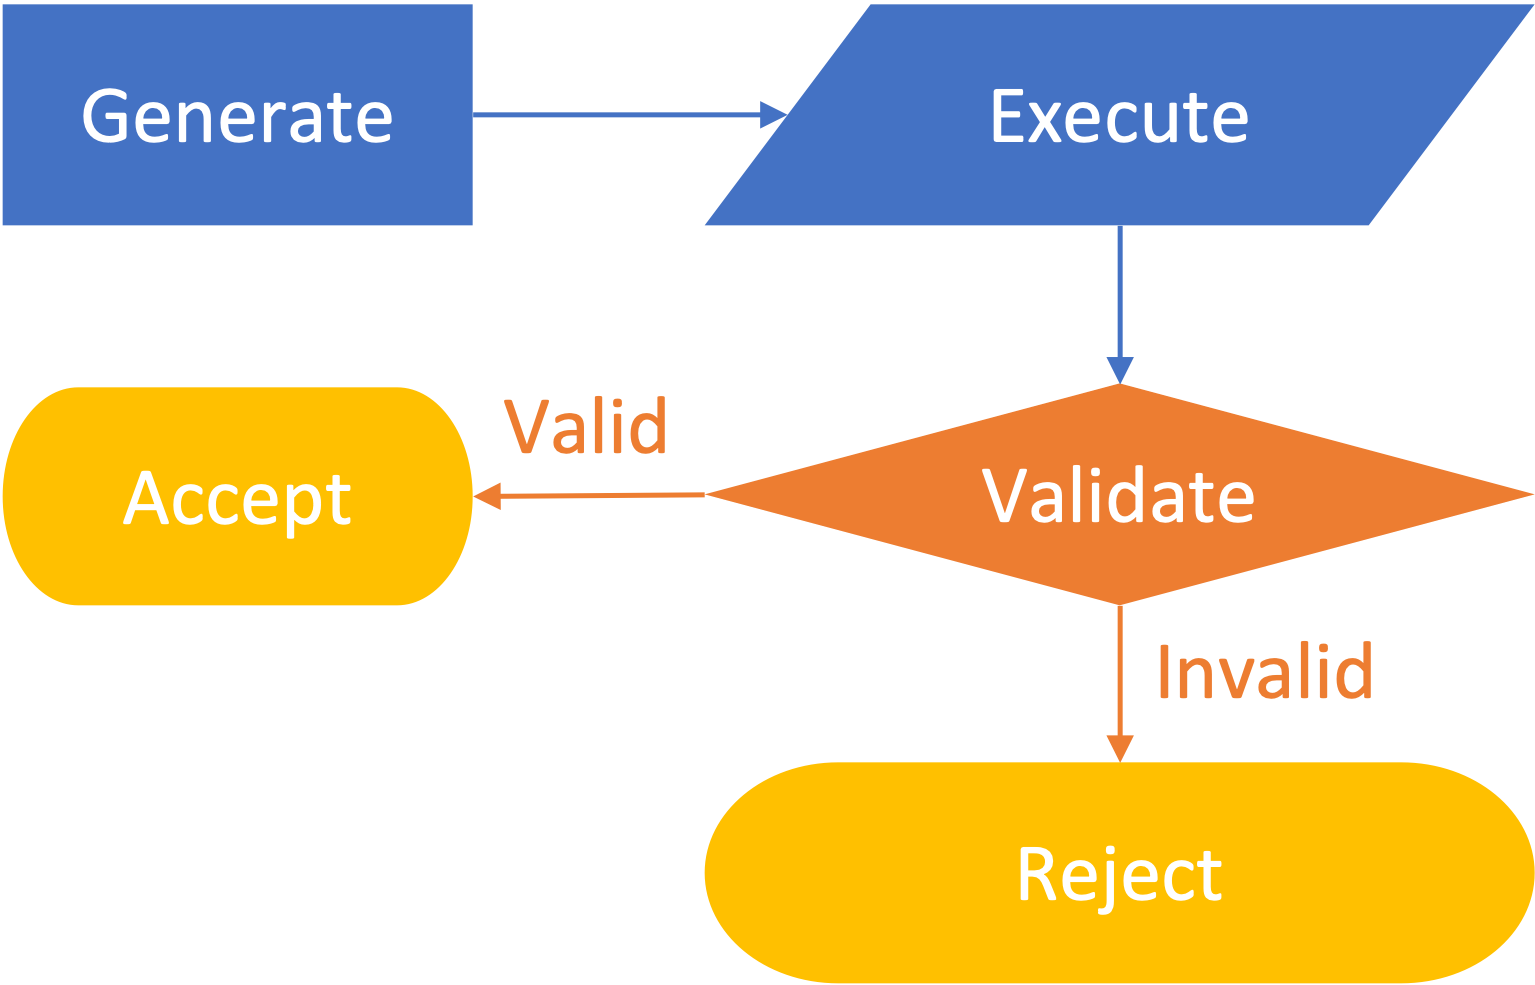
\includegraphics[width=.5\linewidth]{figures/gen-only}
  \caption{Simple tester architecture without shrinking.}
  \label{fig:gen-only}
\end{figure}

However, to achieve better coverage, a randomized generator might produce huge
test input~\cite{Hughes2016}.  Suppose the tester has revealed an invalid
observation after thousands of interactions; such a report provides limited
intuition of where the bug was introduced.  To help developers locate the bug
more effectively, the tester should present a {\em minimal counterexample} that
can reproduce the violation.  This is done by {\em shrinking} the failing input
and rerunning the test with the input's substructures.  As shown
in \autoref{fig:gen-shrink}, if a test input has no substructure that can cause
any failure, then we report it as the minimal counterexample.
\begin{figure}
  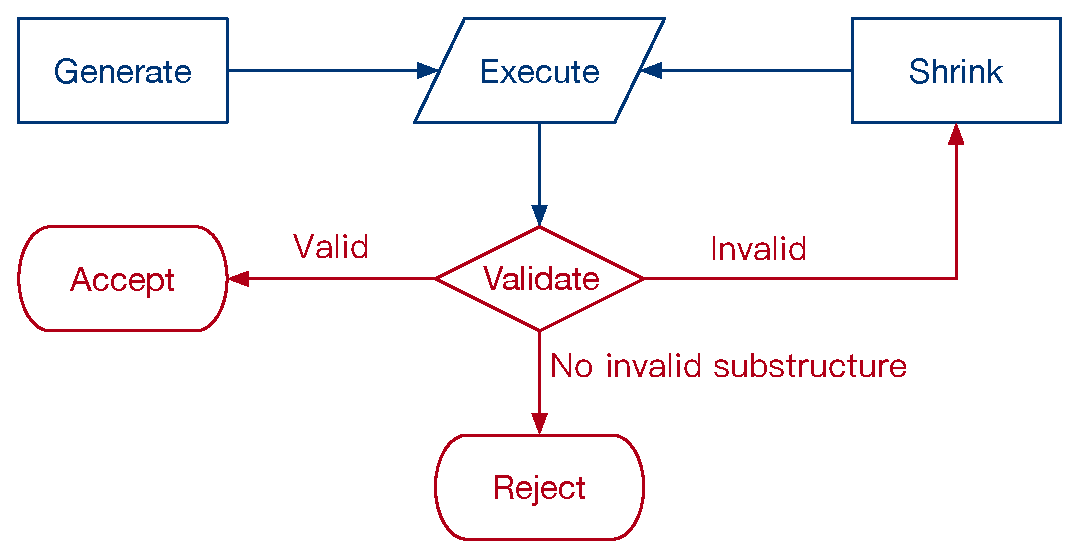
\includegraphics[width=.8\linewidth]{figures/gen-shrink}
  \caption{Tester architecture with shrinking mechanism.}
  \label{fig:gen-shrink}
\end{figure}

The test harness consists of generator, shrinker, and executor.  This thesis
studies the generator and the shrinker that produce the test input.

Interesting test inputs are those that are more likely to reveal invalid
observations.  Such subset is usually sparse and cannot be enumerated within
reasonable budget {\it e.g.} in \autoref{sec:internal-nondeterminism}, request
ETags that match the target resources'.  The tester needs to manipulate the
inputs' distribution, by implementing {\em heuristics} that emphasize certain
input patterns, which is challenged by another form of nondeterminism discussed
as follows.

\subsection{Inter-execution nondeterminism}
\label{sec:inter-execution}
Consider \http, where requests may be conditioned over timestamps.  If a client
has cached a version with a certain timestamp, then it can send the timestamp as
\inlinec{If-Modified-Since} precondition.  The server should not transmit the
request target's content if its \inlinec{Last-Modified} timestamp is not newer
than the precondition's:
\begin{lstlisting}[style=customc,escapeinside={(*}{*)}]
  /* Client: */
  GET /index.html HTTP/1.1
  If-Modified-Since: (*\httpdate\DayAfter[-1]~\currenttime *) GMT
                             /* Server: */
                             HTTP/1.1 200 OK
                             Last-Modified: (*\httpdate\today~\currenttime *) GMT
                             ... content of target ...
  /* Client: */
  GET /index.html HTTP/1.1
  If-Modified-Since: (*\httpdate\today~\currenttime *) GMT
                             /* Server: */
                             HTTP/1.1 304 Not Modified
\end{lstlisting}
In this scenario, an interesting candidate for the \inlinec{If-Modified-Since}
precondition in a test case is the \inlinec{Last-Modified} timestamp of a
previous response.  To emphasize this request pattern, the tester needs to
implement heuristics that generate test inputs based on previous observations.

In case the tester has revealed invalid observations from the server, it needs
to rerun the test with shrunk input.  The timestamps on the server might be
different from the previous execution, so an interesting timestamp in a previous
run might become trivial in this run.

The uncertainty that a system may perform differently among executions is called
{\em inter-execution nondeterminism}.  Such nondeterminism poses challenges to
the input minimization process: To preserve the input pattern, the shrunk \http
request should use the timestamps from the new execution.  We need to implement
a generic shrinking mechanism that can reproduce the heuristics in the test
generator's design.

\section{State of the Art}
\label{sec:existing-work}
This section explains the context for this thesis.  I discuss the state of the
art in the field of testing, and describe their limitations in addressing the
challenges posed by nondeterminism.

\subsection{Property-based testing: QuickCheck}
Property-based testing~\cite{pbt} is a testing methodology for validating
semantic properties of programs' behavior.  The properties are specified as
executable boolean predicates over the behavior.  To check whether an SUT
satisfies a specification, the tester generates test input and executes the SUT
with the generated input.  The tester then observes the SUT's behavior, and
computes the predicates with the observations.

Practices of property-based testing include QuickCheck for Haskell~\cite{qc} and
its variant QuickChick for Coq~\cite{quickchick}.  These tools can generate
random inputs that satisfy logical conditions~\cite{gengood} and integrate with
fuzz testing~\cite{fuzzchick} and combinatorial testing~\cite{judge-cover}, and
have tested real-world systems like telecoms software~\cite{Quviq2006} and
Dropbox~\cite{testing-dropbox}.

\subsection{Model-based testing: TorXakis}
Instead of specifying predicates over systems' behavior, model-based
testing~\cite{mbt} defines an abstract model that produces valid behavior.  When
a tester observes an SUT's behavior, it checks whether the behavior is
producible by the specification model.

Practical tools for model-based testing include TorXakis~\cite{TorXakis}, whose
modelling language is inspired by Language of Temporal Ordering Specification
(LOTOS)~\cite{lotos}, the ISO standard for specifying distributed systems.  The
tool can compile process algebra specifications into tester programs, and can be
used for testing dropbox~\cite{torxakis-dropbox}.

\subsection{Limitations}
In property-based testing, internal and external nondeterminism makes predicates
difficult to write, as discussed
in \autoref{sec:internal-external-nondeterminism}.  TorXakis provides limited
support for internal nondeterminism, allowing the specification to enumerate all
possible values of internal choices.  This works for scenarios where the space
of choices is small {\it e.g.} within a dozen.  When testing ETags
in \autoref{sec:internal-nondeterminism}, it's infeasible to include a list of
all strings in the specification.

To handle inter-execution nondeterminism in QuickCheck, \citet{Hughes2016}
introduced abstract representations for generating and shrinking test inputs
that can adapt to different runtime observations.  His technique works for
synchronous interactions that blocks the tester to wait for observations, and
lacks support for asynchronous testing where the SUT's output may be
indefinitely delayed by the environment.

\section{Contribution}
\label{sec:contribution}
This thesis addresses the challenges in testing caused by various forms of
nondeterminism.  I introduce symbolic languages for specifying the protocol and
representing test input, and {\em dualize} the specification into the tester's
(1) validator, (2) generator, and (3) shrinker:

\begin{enumerate}
\item The specification is written as a reference implementation---a
  nondeterministic program that exhibits all possible behaviors allowed by the
  protocol.  Internal and external nondeterminism are represented by symbolic
  variables, and the space of nondeterministic behavior is defined by all
  possible assignments to the variables.

  For internal nondeterminism, the validator computes the symbolic
  representation of the SUT's output.  The symbolic output expectation is then
  {\em unified} against the tester's observations, reducing the problem of
  validating observations to constraint solving.

  For external nondeterminism, I introduce a model that specifies the
  environment.  The environment model describes the relation between the SUT's
  output and the tester's observations.  By composing the environment model with
  the reference implementation, we get a tester-side specification that defines
  the space of valid observations.
\item Test generation heuristics are defined as computations from observations
  to the next input.  To specify such heuristics in a generic way, I introduce
  intermediate representations for observations and test inputs, which are
  protocol-independent.

  Heuristics in this framework produce symbolic test inputs that are
  parameterized over observations.  During execution, the test harness computes
  the concrete input by {\em instantiating} the symbolic input's arguments with
  runtime observations.
\item The language for test inputs is designed with inter-execution
  nondeterminism in mind.  By instantiating the inputs' symbolic intermediate
  representation with different observations, the test harness gets different
  test inputs but preserves the pattern.

  To minimize counterexamples, the test harness only needs to shrink the inputs'
  symbolic representation.  When rerunning the test, the shrunk input is
  reinstantiated with the new observations, thus reproduces the heuristics by
  the test generator.
\end{enumerate}

\subsection*{Thesis claim}
Symbolic abstract representation can address challenges in testing interactive
systems with uncertain behavior.  Specifying protocols with symbolic reference
implementation enables validating observations of systems with internal and
external nondeterminism.  Representing test input and observations symbolically
allows generating and shrinking interesting test cases despite inter-execution
nondeterminism.  Combining these methods result in a rigorous tester that can
capture protocol violations effectively.

This claim is supported by the following publications:
\begin{enumerate}
\item {\it From C to Interaction Trees: Specifying, Verifying, and Testing a
  Networked Server}~\citep{cpp19}, with Nicolas Koh, Yao Li, Li-yao Xia, Lennart
  Beringer, Wolf Honor\'e, William Mansky, Benjamin C. Pierce, and Steve
  Zdancewic, where I developed a tester program based on a swap server's
  specification written as ITrees~\citep{itree}, and evaluated the tester's
  effectiveness by mutation testing.
\item {\it Verifying an HTTP Key-Value Server with Interaction Trees and
  VST}~\citep{itp21}, with Hengchu Zhang, Wolf Honor\'e, Nicolas Koh, Yao Li,
  Li-yao Xia, Lennart Beringer, William Mansky, Benjamin C. Pierce, and Steve
  Zdancewic, where I developed the top-level specification for \http, and
  derived a tester client that revealed liveness and interrupt-handling bugs in
  our HTTP server, despite it was formally verified.
\item {\it Model-Based Testing of Networked Applications}~\citep{issta21}, which
  describes my technique of specifying \http with symbolic reference
  implementations, and from the specification, automatically deriving a tester
  program that can find bugs in Apache and Nginx.
%% \item {\it Testing by Dualization} (to be submitted to OOPSLA), a theory for
%%   interactive testing, explaining how to specify protocols using abstract model
%%   implementations, and how to guarantee the soundness and completeness of
%%   validators derived from the abstract model.
\end{enumerate}

\subsection*{Outline}
This thesis is structured as follows: \autoref{chap:theory} presents a theory
for synchronous testing, introduces a language family for representing
validators, and shows how to reason about their correctness.
\autoref{chap:dualize} applies the validator theory to an integer machine model,
showing how to derive validators from protocol specifications.
\autoref{chap:itree} transitions from synchronous testing to asynchronous
testing and introduces the ITree specification language.
\autoref{chap:practices} then shows how to derive ITree specifications into
tester programs that can also address external nondeterminism.
\autoref{chap:harness} presents a mechanism for generating and shrinking test
inputs that address inter-execution nondeterminism.  To evaluate the techniques
I proposed in this thesis, \autoref{chap:eval} applies them to testing web
servers and file synchronizers.  I then compare my technique with related works
in \autoref{chap:related-work}, and discuss future directions in
\autoref{chap:discussion}.
